\documentclass{article}

\usepackage{fancyhdr}
\setlength{\headheight}{12pt}
\setlength{\textwidth}{17.2cm} \setlength{\textheight}{23cm}
\setlength{\topmargin}{-2.5cm} \setlength{\headsep}{1.6cm}
\setlength{\evensidemargin}{-.8cm}
\setlength{\oddsidemargin}{-.8cm}
%\pagestyle{fancy}

%set-up page dimentions
\usepackage[top=1 in, bottom = 1 in ,left = 1.5 in, right = 1.5in]{geometry}

\setlength{\parskip}{12pt}  % 12 pt = space between paragraphs
\setlength{\parindent}{12pt} % 0 pt  = indentation
\usepackage{amsmath}
\usepackage{amssymb}
\usepackage{amsthm}
\usepackage{ifthen}
\usepackage{latexsym}
\usepackage{graphicx}
\usepackage{graphics}
\usepackage{psfrag}
\usepackage{graphpap}
\renewcommand{\P}{\text{P}}
\newcommand{\C}{\text{C}}


\newcommand{\natnums}{{\mathbb N}}
\newcommand{\algnums}{{\mathbb A}}
\newcommand{\rationals}{{\mathbb Q}}
\newcommand{\reals}{{\mathbb R}}
\newcommand{\norm}[1]{\left|\left|#1\right|\right|}
\newcommand{\unorm}[1]{{\left|\left|#1\right|\right|_u}}
\newcommand{\scriptR}{\mathcal{R}}
\newcommand{\scriptP}{\mathcal{P}}
\newcommand{\taggedP}{\dot{\mathcal{P}}}
\newcommand{\scriptQ}{\mathcal{Q}}
\newcommand{\taggedQ}{\dot{\mathcal{Q}}}
\newcommand{\pd}{\texttt{PresDroid }}


% Allows hyperlinks if compiled with pdflatex
\usepackage{hyperref}
\hypersetup{colorlinks}
\usepackage{color}
\definecolor{darkred}{rgb}{0.5,0,0}
\definecolor{darkgreen}{rgb}{0,0.5,0}
\definecolor{darkblue}{rgb}{0,0,0.5}
\hypersetup{ colorlinks,
                linkcolor=darkblue,
                filecolor=darkgreen,
                urlcolor=darkblue,
                citecolor=darkblue }
%hyperlink example is: \href{http://www.google.com}{google}

%add code!
\usepackage{listings}
\definecolor{mygreen}{rgb}{0,0.6,0}
\definecolor{mygray}{rgb}{0.5,0.5,0.5}
\definecolor{mymauve}{rgb}{0.58,0,0.82}
\lstset{ %
backgroundcolor=\color{white},   % choose the background color; you must add \usepackage{color} or \usepackage{xcolor}
basicstyle=\footnotesize,        % the size of the fonts that are used for the code
breakatwhitespace=false,         % sets if automatic breaks should only happen at whitespace
breaklines=true,                 % sets automatic line breaking
captionpos=b,                    % sets the caption-position to bottom
commentstyle=\color{mygreen},    % comment style
deletekeywords={...},            % if you want to delete keywords from the given language
escapeinside={\%*}{*)},          % if you want to add LaTeX within your code
extendedchars=true,              % lets you use non-ASCII characters; for 8-bits encodings only, does not work with UTF-8
frame=single,                    % adds a frame around the code
keepspaces=true,                 % keeps spaces in text, useful for keeping indentation of code (possibly needs columns=flexible)
keywordstyle=\color{blue},       % keyword style
language=Octave,                 % the language of the code
morekeywords={*,...},            % if you want to add more keywords to the set
numbers=left,                    % where to put the line-numbers; possible values are (none, left, right)
numbersep=5pt,                   % how far the line-numbers are from the code
numberstyle=\tiny\color{mygray}, % the style that is used for the line-numbers
rulecolor=\color{black},         % if not set, the frame-color may be changed on line-breaks within not-black text (e.g. comments (green here))
showspaces=false,                % show spaces everywhere adding particular underscores; it overrides 'showstringspaces'
showstringspaces=false,          % underline spaces within strings only
showtabs=false,                  % show tabs within strings adding particular underscores
stepnumber=2,                    % the step between two line-numbers. If it's 1, each line will be numbered
stringstyle=\color{mymauve},     % string literal style
tabsize=2,                       % sets default tabsize to 2 spaces
title=\lstname                   % show the filename of files included with \lstinputlisting; also try caption instead of title
}


\begin{document}
\Huge
\begin{center}
    Software Requirements Specification for the \pd\\
    \vspace{3cm}
    \Large
    Angel De Castro\\
    Nicholas Otto\\
    Luis Retana\\
    Christopher Yip\\
    \vspace{2cm}
    Version 0.1\\
    10/4/2013
\end{center}

\normalsize

\newpage
\tableofcontents

\newpage
\section{Introduction}
\subsection{Purpose}
%Identify the product whose software requirements are specified in this document, including the revision or release number. Describe the scope of the product that is covered by this SRS, particularly if this SRS describes only part of the system or a single subsystem.

This document describes the \pd product version 0.1.
\pd aims to facilitate the creation of presentations that can be easily controlled through a simple Android UI. 
This SRS covers the entirety of the \pd project.

%\subsection{Document Conventions}
%Describe any standards or typographical conventions that were followed when writing this SRS, such as fonts or highlighting that have special significance. For example, state whether priorities  for higher-level requirements are assumed to be inherited by detailed requirements, or whether every requirement statement is to have its own priority.

%Todo or takeout

\subsection{Intended Audience} % and Reading Suggestions
%<Describe the different types of reader that the document is intended for, such as developers, project managers, marketing staff, users, testers, and documentation writers. Describe what the rest of this SRS contains and how it is organized. Suggest a sequence for reading the document, beginning with the overview sections and proceeding through the sections that are most pertinent to each reader type.>

\begin{enumerate}
\item Potential User (People wanting to give a presentation)
\item Dr. Pruski
\item Software Development Team
\item Software Testing and Validation Team
\item System Architect
\end{enumerate}

This SRS contains the Product Scope, Overall Description, External Interface Requirements, System Features, Non-Functional Requirements, and Other Requirements of the system. 
The end of the SRS will cover the terms used (Glossary), the models of various aspects of the system (Analysis Models), and aspects of the system to still be determined (To-Be Determined List).

\subsection{Product Scope}
%<Provide a short description of the software being specified and its purpose, including relevant benefits, objectives, and goals. Relate the software to corporate goals or business strategies. If a separate vision and scope document is available, refer to it rather than duplicating its contents here.>
The system will have 2 main components that interact with the user. 
The 1st component is a desktop application that will enable the user to create and display presentations. 
The 2nd component is an Android application that will allow the presenter of the presentation (created via the 1st Component) to control the presentation. 
The presenter will have the following capabilities through the Android application:
\begin{itemize}
\item Scroll/flip through presentation slides
\item Zoom in/out of the presentation
\item Highlight text on the presentation
\item Draw figures on the slides
\item Point to specific content (like a laser pointer) through a simple Android UI and gestures
\end{itemize}


%\subsection{References}
%<List any other documents or Web addresses to which this SRS refers. These may include user interface style guides, contracts, standards, system requirements specifications, use case documents, or a vision and scope document. Provide enough information so that the reader could access a copy of each reference, including title, author, version number, date, and source or location.>

%TODO 

\newpage
\section{Overall Description}
\subsection{Product Perspective}
%<Describe the context and origin of the product being specified in this SRS. For example, state whether this product is a follow-on member of a product family, a replacement for certain existing systems, or a new, self-contained product. If the SRS defines a component of a larger system, relate the requirements of the larger system to the functionality of this software and identify interfaces between the two. A simple diagram that shows the major components of the overall system, subsystem interconnections, and external interfaces can be helpful.>
The \pd is a new stand-alone system that does not depend on any other user systems.  
The desktop application portion will target the Windows and Linux operating system environments.
The mobile application will be targeted for Android mobile phones, specifically Luis' and Angel's phone.

\begin{center}
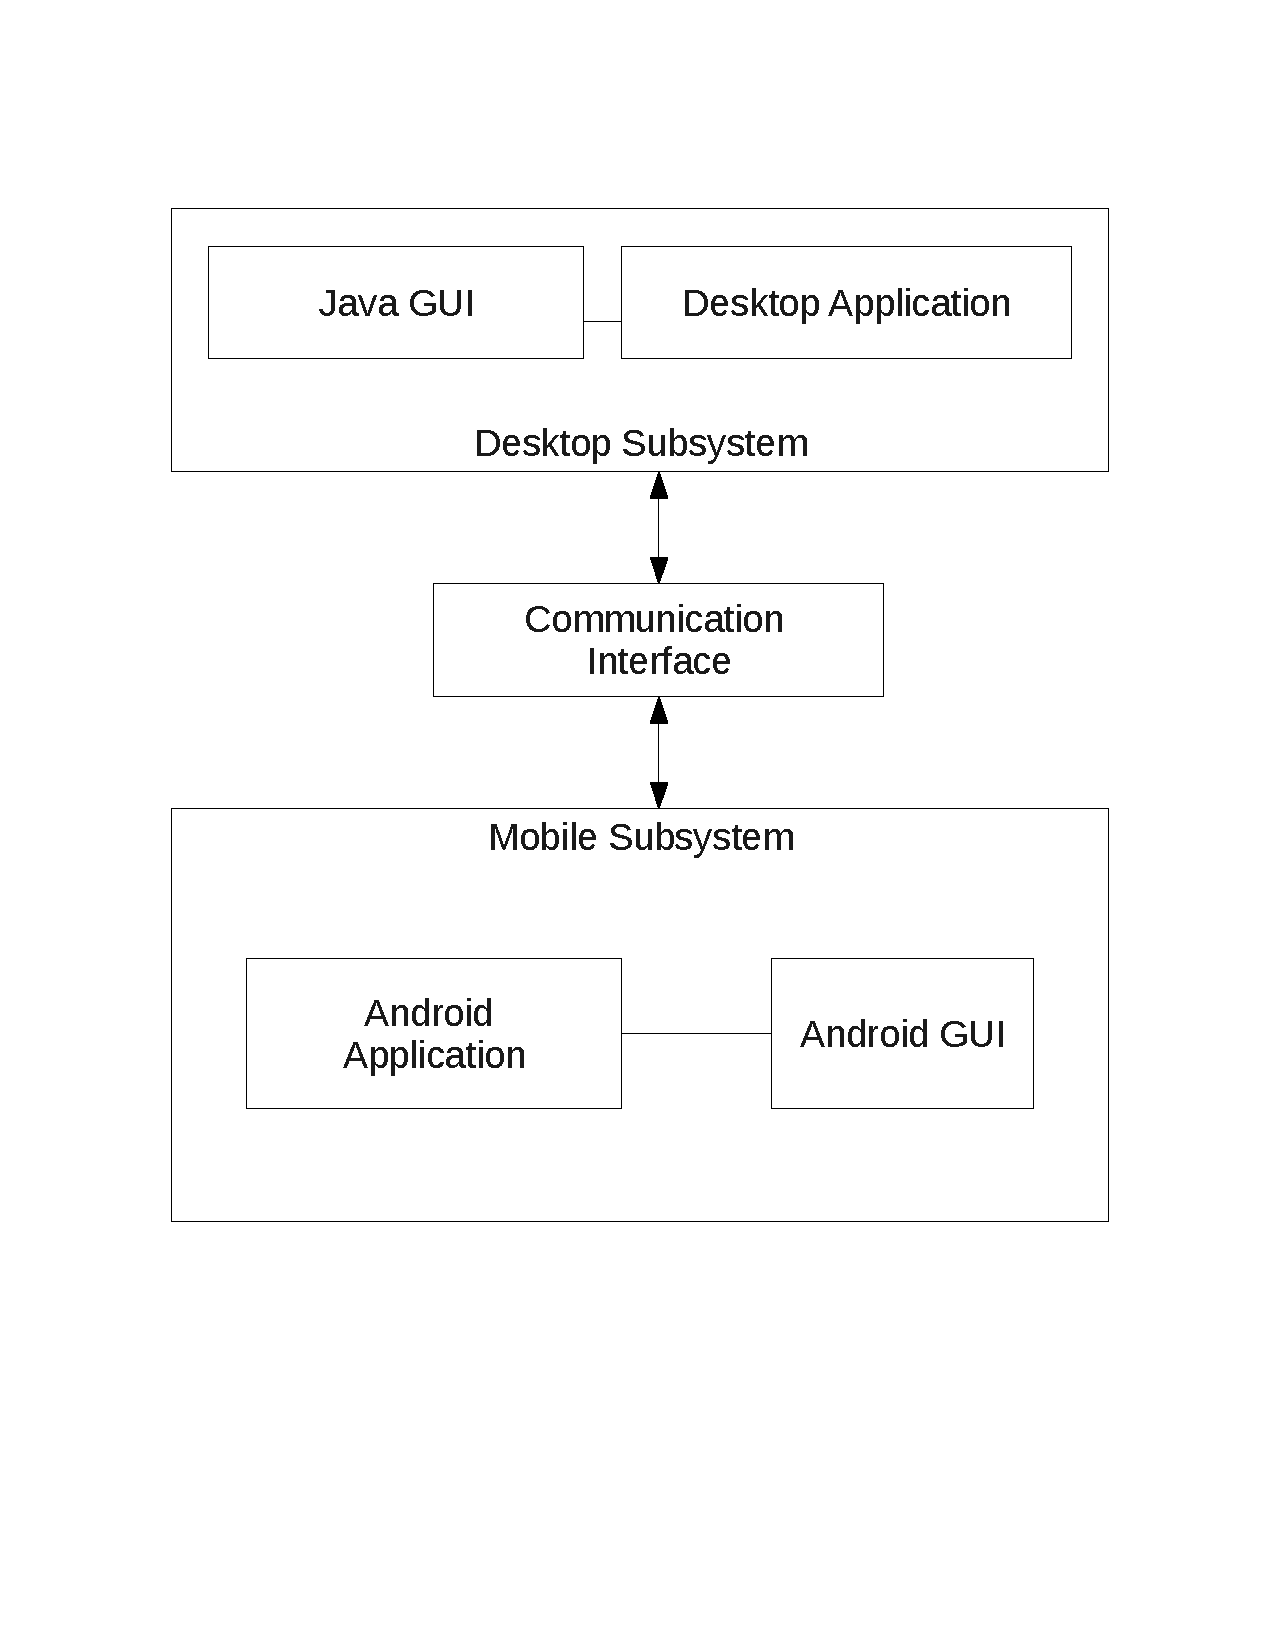
\includegraphics[trim=0cm 5cm 0cm 3cm, clip, scale=0.4]{ppd}
\end{center}

\subsection{Product Functions}
%<Summarize the major functions the product must perform or must let the user perform. Details will be provided in Section 3, so only a high level summary (such as a bullet list) is needed here. Organize the functions to make them understandable to any reader of the SRS. A picture of the major groups of related requirements and how they relate, such as a top level data flow diagram or object class diagram, is often effective.>
The desktop subsystem will perform the following functions:
\begin{itemize}
\item Build a new presentation
\item Present previously built presentation
\item Sync with mobile subsystem
\item Interact with mobile subsystem
\end{itemize}

The mobile subsystem will provide the following functions:
\begin{itemize}
\item Sync with desktop subsystem
\item Accept gesture input
\item Interact with desktop subsystem
\end{itemize}

\subsection{User Classes and Characteristics}
%<Identify the various user classes that you anticipate will use this product. User classes may be differentiated based on frequency of use, subset of product functions used, technical expertise, security or privilege levels, educational level, or experience. Describe the pertinent characteristics of each user class. Certain requirements may pertain only to certain user classes. Distinguish the most important user classes for this product from those who are less important to satisfy.>
The user groups will include students or professors giving simple, quick, and effective presentations.

\subsection{Operating Environment}
%<Describe the environment in which the software will operate, including the hardware platform, operating system and versions, and any other software components or applications with which it must peacefully coexist.>
The hardware requirements for \pd are a Windows or Linux computer where a projector is compatible for the desktop portion and Android mobile phone.
The computer and phone used must have networking (HTTP or Bluetooth, TBD) capabilities.

%\subsection{Design and Implementation Constraints}
%<Describe any items or issues that will limit the options available to the developers. These might include: corporate or regulatory policies; hardware limitations (timing requirements, memory requirements); interfaces to other applications; specific technologies, tools, and databases to be used; parallel operations; language requirements; communications protocols; security considerations; design conventions or programming standards (for example, if the customer’s organization will be responsible for maintaining the delivered software).>
%TODO fill in as we get better idea.

\subsection{User Documentation}
%<List the user documentation components (such as user manuals, on-line help, and tutorials) that will be delivered along with the software. Identify any known user documentation delivery formats or standards.>
User manual.\\
Help section in desktop and mobile application.
\subsection{Assumptions and Dependencies}
%<List any assumed factors (as opposed to known facts) that could affect the requirements stated in the SRS. These could include third-party or commercial components that you plan to use, issues around the development or operating environment, or constraints. The project could be affected if these assumptions are incorrect, are not shared, or change. Also identify any dependencies the project has on external factors, such as software components that you intend to reuse from another project, unless they are already documented elsewhere (for example, in the vision and scope document or the project plan).>
We assume Bluetooth messaging will not be data-constrained and that the computers will have bluetooth messaging capabilities.\\

\newpage
\section{External Interface Requirements}
\subsection{User Interfaces}
%<Describe the logical characteristics of each interface between the software product and the users. This may include sample screen images, any GUI standards or product family style guides that are to be followed, screen layout constraints, standard buttons and functions (e.g., help) that will appear on every screen, keyboard shortcuts, error message display standards, and so on. Define the software components for which a user interface is needed. Details of the user interface design should be documented in a separate user interface specification.>

UI Characteristics for both Desktop and Mobile Applications:
\begin{itemize}
\item The applications will use the GUI Frameworks provided by the system they are built upon. For example, the Mobile application will make use of the native Android GUI Framework (Widgets, Spinners, etc.) while the Desktop Application will make use of the Java Swing Framework (JFrames, JButtons, etc.).
\item The applications must provide a button within the UI which will present the user with a “Help” dialog box or screen.
\item The applications will present errors in two ways:
\begin{itemize}
\item 1) If the error is critical (such as the connection has been lost between the desktop application and mobile application), then a Message/Dialog Box will appear that the user must acknowledge before proceeding.
\item 2) If the error is NOT critical (such as invalid input), then text should appear towards the bottom of the UI in red text to notify the user of a non-critical error occurring.
\end{itemize}
\item The layout of UI elements should adapt to suit to the system that application is installed on. For example, the Android Application UI should be able to adapt to different types of mobile devices (Phone and Tablet) so that elements in the UI don’t appear in unexpected places.
\end{itemize}



\subsection{Hardware Interfaces}
%<Describe the logical and physical characteristics of each interface between the software product and the hardware components of the system. This may include the supported device types, the nature of the data and control interactions between the software and the hardware, and communication protocols to be used.>

The interfaces between both applications and the underlying hardware will be provided through the frameworks used in development such as the Android SDK/Framework and the Java Framework. As mentioned earlier, the supported devices will include Android devices for the Mobile Application and Windows and Linux machines for the desktop application. 

\subsection{Software Interfaces}
%<Describe the connections between this product and other specific software components (name and version), including databases, operating systems, tools, libraries, and integrated commercial components. Identify the data items or messages coming into the system and going out and describe the purpose of each. Describe the services needed and the nature of communications. Refer to documents that describe detailed application programming interface protocols. Identify data that will be shared across software components. If the data sharing mechanism must be implemented in a specific way (for example, use of a global data area in a multitasking operating system), specify this as an implementation constraint.>

Both the Mobile and Desktop subsystems will be built upon Java and Android frameworks, respectively. These frameworks will provide abstract interfaces to operating system features such as file management and multi-threading. Both subsystems (mobile and desktop) will need to create and process a variety of external messages, including, but not limited to:
\begin{itemize}
\item Pair up with mobile or desktop application request
\item Zoom presentation in/out message
\item Move pointer on presentation screen to a specific point message
\item “Kill” connection between desktop and mobile applications message
\end{itemize}

\subsection{Communications Interfaces}
%<Describe the requirements associated with any communications functions required by this product, including e-mail, web browser, network server communications protocols, electronic forms, and so on. Define any pertinent message formatting. Identify any communication standards that will be used, such as FTP or HTTP. Specify any communication security or encryption issues, data transfer rates, and synchronization mechanisms.>

The two major subsystems (as depicted in the “Product Perspective” section above) will communicate using a “Communication Interface”. This Interface will store all messages or requests to be processed and will handle communication between the two subsystems. It will provide a simple and consistent interface where a component can easily check if it has any requests or messages to process. An example of a request is an incoming request for the desktop application (from the Mobile application) to “pair up” with the mobile device so that the two applications can be in sync and can communicate. This “Communication Interface” will need to rely on some form of networking (HTTP, Bluetooth, etc.) to be provided by the host machine. The “Communication Interface” will need to run on a separate thread so that the program will not stall while waiting for incoming messages. The “Communication Interface” must make sure to protect against corruption of its message pool through the use of Semaphores and/or Mutexes, etc.

\newpage
\section{System Features}
Our system needs to communicate two devices, a computer running either Linux or windows, with a portable Android device. The communication is needed so we can control the computer application from the Android device. The computer application will show a simple interface for presentations. The Android device will have to control the change of slides, zoom in/out, writing, moving mouse, go to page and any other function supported by a simple presentation program. If possible we intend to see the pc screen on the Android device. 

\subsection{Communications}
\subsubsection{Description and Priority}
The Android device needs to send and receive data from the computer application. To achieve this goal a communications protocol must be used such as Bluetooth or HTTP. The feature has the highest priority of a 9 since the whole system relies on the Android device communicating with the computer.
\subsubsection{Stimulus/Response Sequences}
This feature must be present from the start, right after the user turns both devices on.  The moment the devices are switched on they must be able to communicate with each other so the normal use of the application can continue
\subsubsection{Functional Requirements}
The communications must be robust, the state of the link must be constantly checked so there is no down time. In case of loss of communications the system must be able to create a new channel of communication. If this fails the user must be prompted of the error.

\subsection{Synchronization}
\subsubsection{Description and Priority}
Before any other function becomes available we need to synchronize the Android device with the computer. This must be done by selecting in both machines the sync button. Once both devices find each other they can pair up. The feature has the highest priority of a 9 since the whole system relies on the Android device maintaining a link with computer
\subsubsection{Stimulus/Response Sequences}
This feature must be present from the start, right after the user turns both devices on. Once on, the first task to complete must be a successful synchronization, so the normal use of the application can continue. To accomplish this link both devices must be searching for a pair, once found they can create the link.
\subsubsection{Functional Requirements}
The link must be robust, the state of the link must be constantly checked so there is no down time. For these checks any package sent must receive a confirmation package.  If data fails to reach its destination the system must resend the package. In case of complete loss of the link, the system must be able search for the same device to try and reconnect automatically. If this fails the user must be prompted of the failure.
\subsection{Android Gestures}
\subsubsection{Description and Priority}
The Android Application must be able to accept input from the user by hand gestures. Using the Androids touch screen the user will send commands to the Android application. These commands must be then sent to the computer were they will be processed and a task will be executed. Such tasks will include the passing of slides, zoom in/out, moving the mouse, etc. This is feature is of the highest priority 9, since it’s the core function of the system.
\subsubsection{Stimulus/Response Sequences}
After both applications have synced this feature must be made available, a drawn gesture on the Android application must be directly followed by an action in the computer application.
\subsubsection{Functional Requirements}
This feature must be robust and responsive with no lag. Any input into the Android device must be immediately show on the computer screen. This way the user gets a feeling of complete control and responsiveness. In case of an error the user will be prompted with a message to repeat the gesture.
\subsection{Simple Presentation Interface on Computer}
\subsubsection{Description and Priority}
The task of the computer application is to function as a presentation GUI, it must be able to open and create presentation showing them on screen. The priority of this feature is the highest 9, since all future features rely on it, needing it as a visual interface.
\subsubsection{Stimulus/Response Sequences}
The presentation interface must appear once both applications have been synchronized, the screen must reflect the changes from any input the user sends through the Android device screen.
\subsubsection{Functional Requirements}
Should be a robust and reliable program, it's controlled by gestures through the Android device so the inputs will be largely varied and vague.
\subsection{Computer Screen on Android Device}
\subsubsection{Description and Priority}
Instead of having a specific Android interface the computer screen could be shown on the Android device. This way the user can select or underline exactly were intended without the need of a mouse cursor. This also makes it easier for the user to change slides or zoom in/out at specific points. This feature has a priority of 5, it's not essential for the system it simply makes it more interactive. 
\subsubsection{Stimulus/Response Sequences}
The presentation must appear on the Android device once both applications have been synchronized, the screen must reflect the changes from any input the user sends through the Android device screen.
\subsubsection{Functional Requirements}
Should be robust and reliable, it's controlled by gestures through the Android device so the inputs will be largely varied and vague.

%<This template illustrates organizing the functional requirements for the product by system features, the major services provided by the product. You may prefer to organize this section by use case, mode of operation, user class, object class, functional hierarchy, or combinations of these, whatever makes the most logical sense for your product.>

%\subsection{System Feature 1}
%<Don’t really say “System Feature 1.” State the feature name in just a few words.>
%\subsubsection{Description and Priority}
%<Provide a short description of the feature and indicate whether it is of High, Medium, or Low priority. You could also include specific priority component ratings, such as benefit, penalty, cost, and risk (each rated on a relative scale from a low of 1 to a high of 9).>

%\subsubsection{Stimulus/Response Sequences}
%<List the sequences of user actions and system responses that stimulate the behavior defined for this feature. These will correspond to the dialog elements associated with use cases.>

%\subsubsection{Functional Requirements}
%<Itemize the detailed functional requirements associated with this feature. These are the software capabilities that must be present in order for the user to carry out the services provided by the feature, or to execute the use case. Include how the product should respond to anticipated error conditions or invalid inputs. Requirements should be concise, complete, unambiguous, verifiable, and necessary. Use “TBD” as a placeholder to indicate when necessary information is not yet available.>

%<Each requirement should be uniquely identified with a sequence number or a meaningful tag of some kind.>
\newpage
\section{Other Nonfunctional Requirements}
\subsection{Performance Requirements}
%<If there are performance requirements for the product under various circumstances, state them here and explain their rationale, to help the developers understand the intent and make suitable design choices. Specify the timing relationships for real time systems. Make such requirements as specific as possible. You may need to state performance requirements for individual functional requirements or features.>
\subsubsection{Mobile to Desktop Communication}
The delay between user interaction on mobile device and registration of user action on the desktop environment should be minimized.
\begin{enumerate}
    \item Requirement Completely Met: Mobile to desktop communication appears instantaneous.
    \item Acceptable: The mobile to desktop communication contains predictable lag that does not distract user performance.
    \item Not Met: The user is unable to compensate for inconsistencies or poor mobile to desktop communication performance.
\end{enumerate}

\subsubsection{Syncing of Mobile to Desktop}
The time it takes to sync the mobile device to the desktop suite should be less than 4 seconds.

\subsubsection{Desktop Program Start-Up}
The time it takes to start the desktop suite should be less than 8 seconds.

\subsubsection{Desktop Program Response}
The presentation creation program should have negligible response times accepting and displaying user input.

\subsection{Safety Requirements}
%<Specify those requirements that are concerned with possible loss, damage, or harm that could result from the use of the product. Define any safeguards or actions that must be taken, as well as actions that must be prevented. Refer to any external policies or regulations that state safety issues that affect the product’s design or use. Define any safety certifications that must be satisfied.>
There are no known physical safety requirements at this time.  Caution should be exercised when using any unfamiliar device, however.\\

The desktop suite shall not modify any user files other than the files currently opened by the user.
Furthermore, the desktop suite shall perform an "auto-save" while the user modifying a presentation.  These auto-saves will occur once every 5 minutes.
\subsection{Security Requirements}
%<Specify any requirements regarding security or privacy issues surrounding use of the product or protection of the data used or created by the product. Define any user identity authentication requirements. Refer to any external policies or regulations containing security issues that affect the product. Define any security or privacy certifications that must be satisfied.>
\begin{itemize}
    \item Each presentation will only allow syncing to one mobile device.
    \item A mobile device will not disconnect another mobile device from its connection to the desktop suite.
    \item A desktop will not automatically sync with a mobile device.
    \item Requests made outside of standard mobile to desktop interface will return a standard error message.
\end{itemize}
NO requirement is given that communication needs to be encrypted.\\

\subsection{Software Quality Attributes}
%<Specify any additional quality characteristics for the product that will be important to either the customers or the developers. Some to consider are: adaptability, availability, correctness, flexibility, interoperability, maintainability, portability, reliability, reusability, robustness, testability, and usability. Write these to be specific, quantitative, and verifiable when possible. At the least, clarify the relative preferences for various attributes, such as ease of use over ease of learning.>
The source code will adhere to the following attributes:
\begin{itemize}
    \item The source code will be reasonably documented.  All non-trivial functions or methods will have header documentation describing the following:
        \begin{enumerate}
            \item Name
            \item General description, including pre-conditions
            \item List and description of input parameters
            \item List and description of returned values
            \item Information about state change during method execution (post-condition)
        \end{enumerate}
    \item The source code will adhere to a single programming style, namely the Stroustrup variant of K\&R style.
    \item All code blocks will be enclosed in curly brackets, even if not explicitly required.
\end{itemize}

Above all else, the system will strive to be usable.  We want flexibility, but if rigid assumptions must be made to release the product on time, then so be it.



\subsection{Business Rules}
%<List any operating principles about the product, such as which individuals or roles can perform which functions under specific circumstances. These are not functional requirements in themselves, but they may imply certain functional requirements to enforce the rules.>
This product will ship by the end of the fall semester.


\newpage
%\section{Other Requirements}
%<Define any other requirements not covered elsewhere in the SRS. This might include database requirements, internationalization requirements, legal requirements, reuse objectives for the project, and so on. Add any new sections that are pertinent to the project.>


%\section{Appendix A: Glossary}
%<Define all the terms necessary to properly interpret the SRS, including acronyms and abbreviations. You may wish to build a separate glossary that spans multiple projects or the entire organization, and just include terms specific to a single project in each SRS.>


%\section{Appendix B: Analysis Models}
%<Optionally, include any pertinent analysis models, such as data flow diagrams, class diagrams, state-transition diagrams, or entity-relationship diagrams.>


%\section{Appendix C: To Be Determined List}
%<Collect a numbered list of the TBD (to be determined) references that remain in the SRS so they can be tracked to closure.>

\end{document}
